\sectionquestion{Optimization, Regularization, and Modeling}

\begin{parts}
\part Suppose you are given a dataset of $N$ data points $(x^{(i)},y^{(i)})_{i=1}^N$ where $x^{(i)},y^{(i)} \in \mathbb{R}$ and you fit a linear regression model to this dataset with no bias term and L2 regularization, i.e., you minimize the following objective function for:
\begin{equation*}
    J(\theta) = \frac{1}{N} \sum_{i=1}^n \left(\frac{1}{2} \left(y^{(i)}-\theta x^{(i)}\right)^2 \right) + \frac{\lambda}{2} \theta^2
\end{equation*}

\begin{subparts}
    \subpart[2] \textbf{Math:} What is $\frac{\partial J(\theta)}{\partial \theta}$? \textbf{You do not need to show your work for this problem.}
    \begin{tcolorbox}[fit,height=4cm, width=15cm, blank, borderline={1pt}{-2pt}]
        \begin{soln}
            \begin{equation*}
                \frac{\partial J(\theta)}{\partial \theta} = \frac{1}{N} \left(\sum_{i=1}^N \left(\theta {x^{(i)}}^2- x^{(i)} y^{(i)}\right)\right) + \lambda \theta
            \end{equation*}
        \end{soln}
    \end{tcolorbox}
        
    \subpart[2] \textbf{Math:} Find the closed form solution for $\hat{\theta}$, the optimal value of $\theta$. \textbf{Again, you do not need to show your work for this problem.}
    \begin{tcolorbox}[fit,height=4cm, width=15cm, blank, borderline={1pt}{-2pt}]
        \begin{soln}
            \begin{equation*}
                \hat{\theta} = \frac{\sum_{i=1}^N x^{(i)}y^{(i)}}{\sum_{i=1}^N {x^{(i)}}^2 + N\lambda}
            \end{equation*}
        \end{soln}
    \end{tcolorbox}
    
    \subpart[2] \textbf{Drawing:} Suppose you train several linear regression models on the same dataset with different values of $\lambda$. On the axes provided below, draw a curve that depicts the general trend you would expect $|\hat{\theta}|$ to follow as $\lambda$ increases.  
    
    \centering
    \begin{tikzpicture}
    \begin{axis}[
        scale=0.9,
        xlabel={\Large $\lambda$},
        ylabel={\Large $|\hat{\theta}|$},
        xmin=1,
        xmax=20,
        ymin=1,
        ymax=20,
        xticklabels={,,},
        yticklabels={,,},
        % domain=0:5,
        samples=100,
        axis lines=middle,
        enlargelimits=true
    ]
    \begin{comment}
        % y=1
        \addplot[blue, thick] {0.5} node[pos=0.85, above] {(1)};
        
        % y=e^x
        \addplot[red, thick] {exp(-x)} node[pos=0.85, above] {(2)};
        
        % y=1-e^x
        \addplot[green, thick] {1-exp(-x)} node[pos=0.85, above] {(3)};
    
        \addplot[black, thick] {1-x/5} node[pos=0.85, above] {(4)};
        \end{comment}
        \end{axis}
    \end{tikzpicture}
    
    \begin{soln}
        Curve should look something like $\theta = \frac{1}{\lambda}$
    \end{soln}
\end{subparts}
\begin{qauthor}
    Pranit, Linear Regression

    Lightly edited by Henry
\end{qauthor}

\part Consider the following toy dataset with two data points. Each data point has two features, $X_1$ and $X_2$, and a label $Y$.
\begin{center}
    \begin{tabular}{|c|c|c|c|}
    \hline 
    $i$ & $X_1$ & $X_2$ & $Y$ \\ \hline
    1 & 1 & 0 & 1 \\ \hline 
    2 & -1 & 1 & 2 \\ \hline 
    \end{tabular}
\end{center}
You are interested in minimizing the objective function $J(\thetav)=\frac{1}{N}\sum_{i=1}^N J^{(i)}(\thetav)$, where $N$ is the number of data points and 
$$J^{(i)}(\thetav) = \frac{1}{2}y^{(i)}\left(\thetav^T\xv^{(i)}\right)^{2}$$
Suppose $\thetav$, the parameter vector, is initialized to $\begin{bmatrix} 2 \\ 1 \end{bmatrix}$.

\begin{subparts}
\subpart[1] \textbf{Numerical Answer:} For the toy dataset above, what does the objective function evaluate to at initialization? 
\begin{tcolorbox}[fit,height=1.5cm, width=3cm, blank, borderline={1pt}{-2pt}]
    \begin{soln}
        For $x^{(1)}$: 4/2 = 2
        For $x^{(2)}$: 1
        Ans: 1.5
    \end{soln}
\end{tcolorbox}

\subpart[2] \textbf{Math:} Let's use stochastic gradient descent to find the optimal value of $\thetav$: what is the gradient of $J^{(i)}$ with respect to $\theta_j$? 

$\frac{ \partial J^{(i)}(\thetav) }{ \partial \theta_j}=$  \begin{tcolorbox}[fit,height=1.5cm, width=6cm, blank, borderline={1pt}{-2pt}, nobeforeafter]
    \begin{soln}
        $y^{(i)}(\thetav^T\xv^{(i)})\xv^{(i)}_j$
    \end{soln}
\end{tcolorbox} 

\subpart[2] \textbf{Numerical Answer:} Perform one epoch of stochastic gradient descent, using each data point in the order presented in the table. Use the initialization $\theta = \begin{bmatrix} 2 \\ 1 \end{bmatrix}$ and assume a learning rate of $\alpha=1$. 

What is the updated parameter vector $\thetav$?
\\ \\
$\theta_1$ = \begin{tcolorbox}[fit,height=1.5cm, width=3cm, blank, borderline={1pt}{-2pt}, nobeforeafter]
    \begin{soln}
        $2$
    \end{soln}
\end{tcolorbox}

$\theta_2$ = \begin{tcolorbox}[fit,height=1.5cm, width=3cm, blank, borderline={1pt}{-2pt}, nobeforeafter]
    \begin{soln}
        $-1$
    \end{soln}
\end{tcolorbox}

\begin{soln}
    After first update: [2 - 1*1*2, 1 - 1*0*1] = [0,1]
    After second update: [0 - 1*2*-1, 1 - 1*2*1]  = [2, -1]
\end{soln}

\begin{comment}
\subpart[1]{}
For the given toy dataset, what does the objective function evaluate to with the updated theta? 

    \begin{tcolorbox}[fit,height=1cm, width=2cm, blank, borderline={1pt}{-2pt}]
    %solution
    \end{tcolorbox}
    \begin{soln}
    For point 1: 0
    For point 2: 2
    Ans: 1
    \end{soln}   
\end{comment}  

\end{subparts}    
\begin{qauthor}
    Tanvi, Apply stochastic gradient descent (SGD) to optimize a function

    Edited by Henry, love this question
\end{qauthor}

\begin{comment}
\part[1] \textbf{Select all that apply:} Neural is training a linear regression model to predict the prices of houses in Pittsburgh with L0 regularization of all terms including the bias term. He finds that his model has a very high error on the test data, but a low error on the train data. Which of the following apply?
    {%
    \checkboxchar{$\Box$} \checkedchar{$\blacksquare$} % change checkbox style locally
    \begin{checkboxes}
     \choice Using the test data to train would cause the error on the test data to decrease.
     \choice It is a good idea to use the test data to train, because the model will generalize well and decrease the true error.
     \choice As L0 regularization drives more terms to zero, suggest that Neural use L1 regularization instead of L0 regularization to avoid driving the bias term to zero.
     \choice Suggest that Neural not regularize the bias term at all.
    \end{checkboxes}
    }
    \begin{soln}
    A, D.
    \end{soln}
    \begin{qauthor}
    Tanvi, Explain why we should not regularize the bias term. [MCQ form]. Also incorporate parts of distinguishing between true and test error.
    
    Removed by Henry; I like the Short answer form of the question better!
    \end{qauthor}
\end{comment}

\newpage
\part[2] \textbf{Short Answer:} Neural the Narwhal is training a linear regression model to predict housing prices in Pittsburgh. He uses L0 regularization on all of the parameters, \emph{including the bias term}. He finds that his model has a very high error rate on his test dataset, but a low error on the train data. Graddyant suggests that he perform L1 regularization on the bias term, since L0 regularization tends to drive terms to zero, and the bias term should not be zero. Is this an appropriate suggestion? Briefly justify your answer in 2-3 concise sentences. 
\fillwithlines{9em}
\begin{soln}
    No, the bias term should not be regularized at all because the value of the bias term captures a fundamental property of the data and not the importance of certain features. It is alright for the bias to be zero.
\end{soln}
\begin{qauthor}
    Tanvi, Explain why we should not regularize the bias term. [Short answer form]

    Lightly edited by Henry
\end{qauthor}
    
\begin{comment}
\part[2] \textbf{Short answer:} Describe an effective strategy used to balance between error and model complexity. What are its effects on error and complexity?
\fillwithlines{6em}
\begin{soln}
    Regularization helps to reduce dimensionality by reducing the weight of particular features. As a result, we decrease our complexity ($\mathcal{VC(H)}$) and be able to better generalize to unseen examples. However, a higher dimensionality (more features) allows us to better fit to the training data and lower our error. Regularization might result in slight increases in our training error.
\end{soln}
\begin{qauthor}
Sebastian

Removed by Henry: I like what this question is getting at but it's a bit vague as currently written. 
\end{qauthor}
\end{comment}



\begin{comment}
\begin{subparts}
    \subpart[2] \textbf{Numerical Answer:} Use the Finite Difference Method to approximate the derivative of the function at $x = 2$ with $\epsilon = 1$. \textbf{For full credit you must show all your work.}
    
    \begin{tcolorbox}[fit,height=4cm, width=15cm, blank, borderline={1pt}{-2pt}]
        \begin{soln}
        Depending on the formula used, accept both
        \[ f'(2) \approx \frac{f(2 + 1) - f(2)}{1} = 38 - 21 = 17\] 
        \[ f'(2) \approx \frac{f(2 + 1) - f(2 - 1)}{2} = \frac{38 - 10}{2} = 14\] 
        \end{soln}
    \end{tcolorbox}
    
    \subpart[2] \textbf{Short Answer:} Without referencing the exact value of the derivative at $x = 2$, do you think the estimate you computed in the previous part is a good estimate? Briefly justify your answer in 1-2 concise sentences. 
    \fillwithlines{6em}
    \begin{soln}
        Probably not no, the value of $\epsilon$ used is very large
    \end{soln}
\end{subparts}
\end{comment}
\begin{qauthor}
    Yash, Use the finite difference method to evaluate the gradient of a function

    Edited by Henry
\end{qauthor}
    
\begin{comment}
   \part[1] \textit{Fill in the blank:} For a \underline{\hspace{3em}} function, every local minimum is a global minimum. \textbf{Select all that apply.}
    {%
    \checkboxchar{$\Box$} \checkedchar{$\blacksquare$} % change checkbox style locally
    \begin{checkboxes}
     \choice convex
     \choice strictly convex
     \choice nonconvex
     \choice None of the above
    \end{checkboxes}
    }
    \begin{soln}
    convex, strictly convex
    \end{soln}
    \begin{qauthor}
        Abhi
        Distinguish between convex, concave, and nonconvex functions
    \end{qauthor}
    
\part [1] \textbf{Short answer:} Neural designs a loss function which is twice differentiable and not convex, but decides to use gradient descent to optimize it anyway. Is it possible that gradient descent might converge to a local maxima instead of a local minima? Explain your answer in one sentence.
    \fillwithlines{6em}
    \begin{soln}
       Yes, if the algorithm initializes at a local maxima. 
    \end{soln}

    \begin{qauthor}
    Pranit, Distinguish between convex, concave, and nonconvex functions
    \end{qauthor}

    
    \begin{qtester}
     nice!
    \end{qtester}



\part[2] \textbf{Select all that apply:} 
Suppose we are performing binary classification on a 1-dimensional labelled dataset consisting of three points as described in the table below. Which of the following feature transformations $f(x)$ would make the data linearly separable?

\begin{minipage}{0.4\linewidth}
\begin{table}[H]
    \centering
    \begin{tabular}{c|c}
    data point $x$ & label $y$ \\
    \hline
    $-\pi$ & 1 \\
    0 & 0 \\
    $\frac{\pi}{2}$ & 1
    \end{tabular}
    \label{tab:my_label}
\end{table}
\end{minipage}
%
\begin{minipage}{0.6\linewidth}
% Adapted from: https://tex.stackexchange.com/questions/249953/locating-tick-marks-at-integral-multiples-of-pi-2
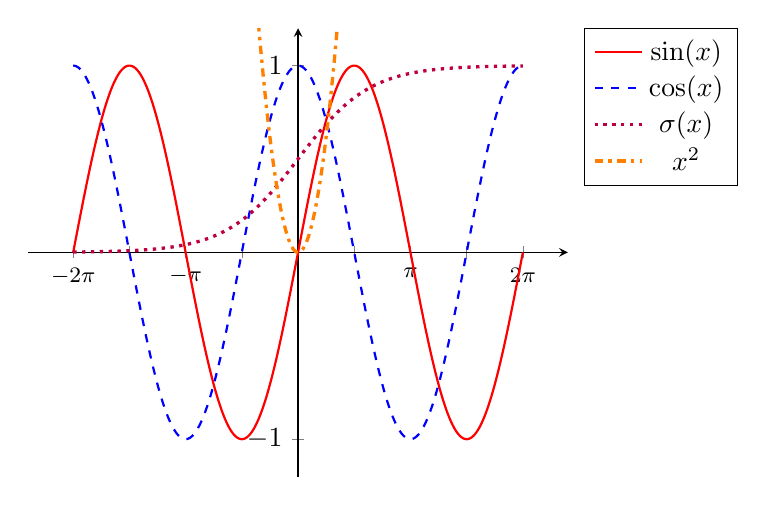
\begin{tikzpicture}
    \begin{axis}[
        legend pos=outer north east,
        xtick={-2*pi, -(3/2)*pi, -pi, -(1/2)*pi, (1/2)*pi, pi, (3/2)*pi, 2*pi},
        %        xtick={-6.28318, -4.7123889, -3.14159, -1.5708, 1.5708, 3.14159, 4.7123889, 6.28318},
        xticklabel style={font=\footnotesize,fill=white},
        xticklabels={$-2\pi$,,$-\pi$,,,$\pi$,,$2\pi$},
        ytick={-1,1},
        axis lines=middle,
        domain=-2*pi:2*pi,
        samples=501,
        enlargelimits=true,
        ymax=1, ymin=-1,
        ]
    \addplot[thick, solid, red] {sin(deg(x))};
    \addplot[thick, dashed,blue] {cos(deg(x))};
    \addplot[very thick, dotted,purple] {1/(1+ exp(-x))};
    \addplot[very thick, dashdotted,orange] {x^2};
    \legend{$\sin(x)$,$\cos(x)$,$\sigma(x)$,$x^2$}
    \end{axis}
\end{tikzpicture}
\end{minipage}

{%
    \checkboxchar{$\Box$} \checkedchar{$\blacksquare$} % change checkbox style locally
    \begin{checkboxes}
     \choice $f(x) = \sin(x)$
     \choice $f(x) = \cos(x)$
     \choice $f(x) = \sigma(x)$
     \choice $f(x) = x^2$
     \choice None of the above
    \end{checkboxes}
}
\begin{soln}
    B, D
\end{soln}
\begin{qauthor}
    Alex, Convert linearly inseparable dataset to a linearly separable dataset in higher
dimensions. Matt, added plot.
\end{qauthor}

\begin{qtester}
I like this question.
\end{qtester}


\part Neural creates a linear regression model $M_1$ for work, but his boss Markov tells him that $M_1$ uses too many features 
% COMMENTING OUT TO NOT GIVE THINGS AWAY: 
% (i.e., has too many features with nonzero coefficients) 
to be easily explained. He decides to use ridge regression (L2 regularization) to identify and remove irrelevant features. Neural trains a new model using ridge regression, then removes every feature with a weight of exactly $0$ from his model---he dubs the result $M_2$. However, $M_2$ still uses the same number of features as $M_1$ after this process (i.e., no features were removed).

\begin{subparts}
    \subpart[1] \textbf{Short answer:} Explain why the feature removal process was not effective at getting rid of features.
    \fillwithlines{6em}
    \begin{soln}
    L2 penalty doesn't push many parameters to $0$, can leave them at very small values. They won't get removed in step 2.
    \end{soln}

    \subpart[1] \textbf{Short answer:} Describe an alternative method of feature selection using $L2$ regularization that would reliably get rid of some features.
    \fillwithlines{6em}
    \begin{soln}
        L2 but remove the $k$ features with smallest weight, instead of only exactly 0
    \end{soln}

    \subpart[1] \textbf{Short answer:} Describe a method of feature selection via another form of regularization that Neural could use.
    \fillwithlines{6em}
    \begin{soln}
    LASSO
    \end{soln}
\end{subparts}
    \begin{qauthor}
    Abhi, Use feature selection techniques to identify and remove irrelevant features
    \end{qauthor}
\begin{qtester}
I like this question. I suspect we will get some creative answers about why it was not effective, but that's probably ok.
\end{qtester}     
\end{comment}
\end{parts}